\section{Method}
	\subsection{Hardware}
		\subsubsection{\gls{uwb} transceiver module — DWM1000}
			\begin{figure}[H] 
			  \centering
			      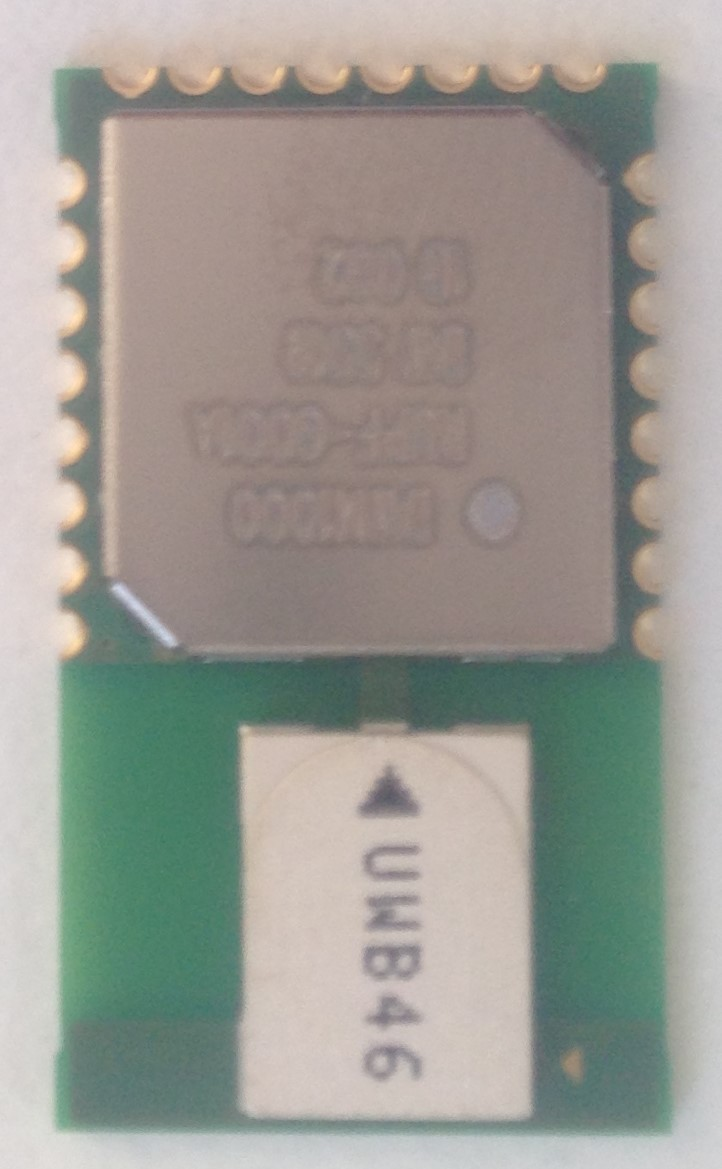
\includegraphics[height=0.45\textwidth, angle=180]{img/UWB-module}
			  \caption{One of the DWM1000 \gls{uwb} modules from Decawave used in the project.}
			  \label{fig_DWM1000}
			\end{figure}
		\subsubsection{Wireless sensor module — Tmote Sky}
			\begin{figure}[H] 
			  \centering
			      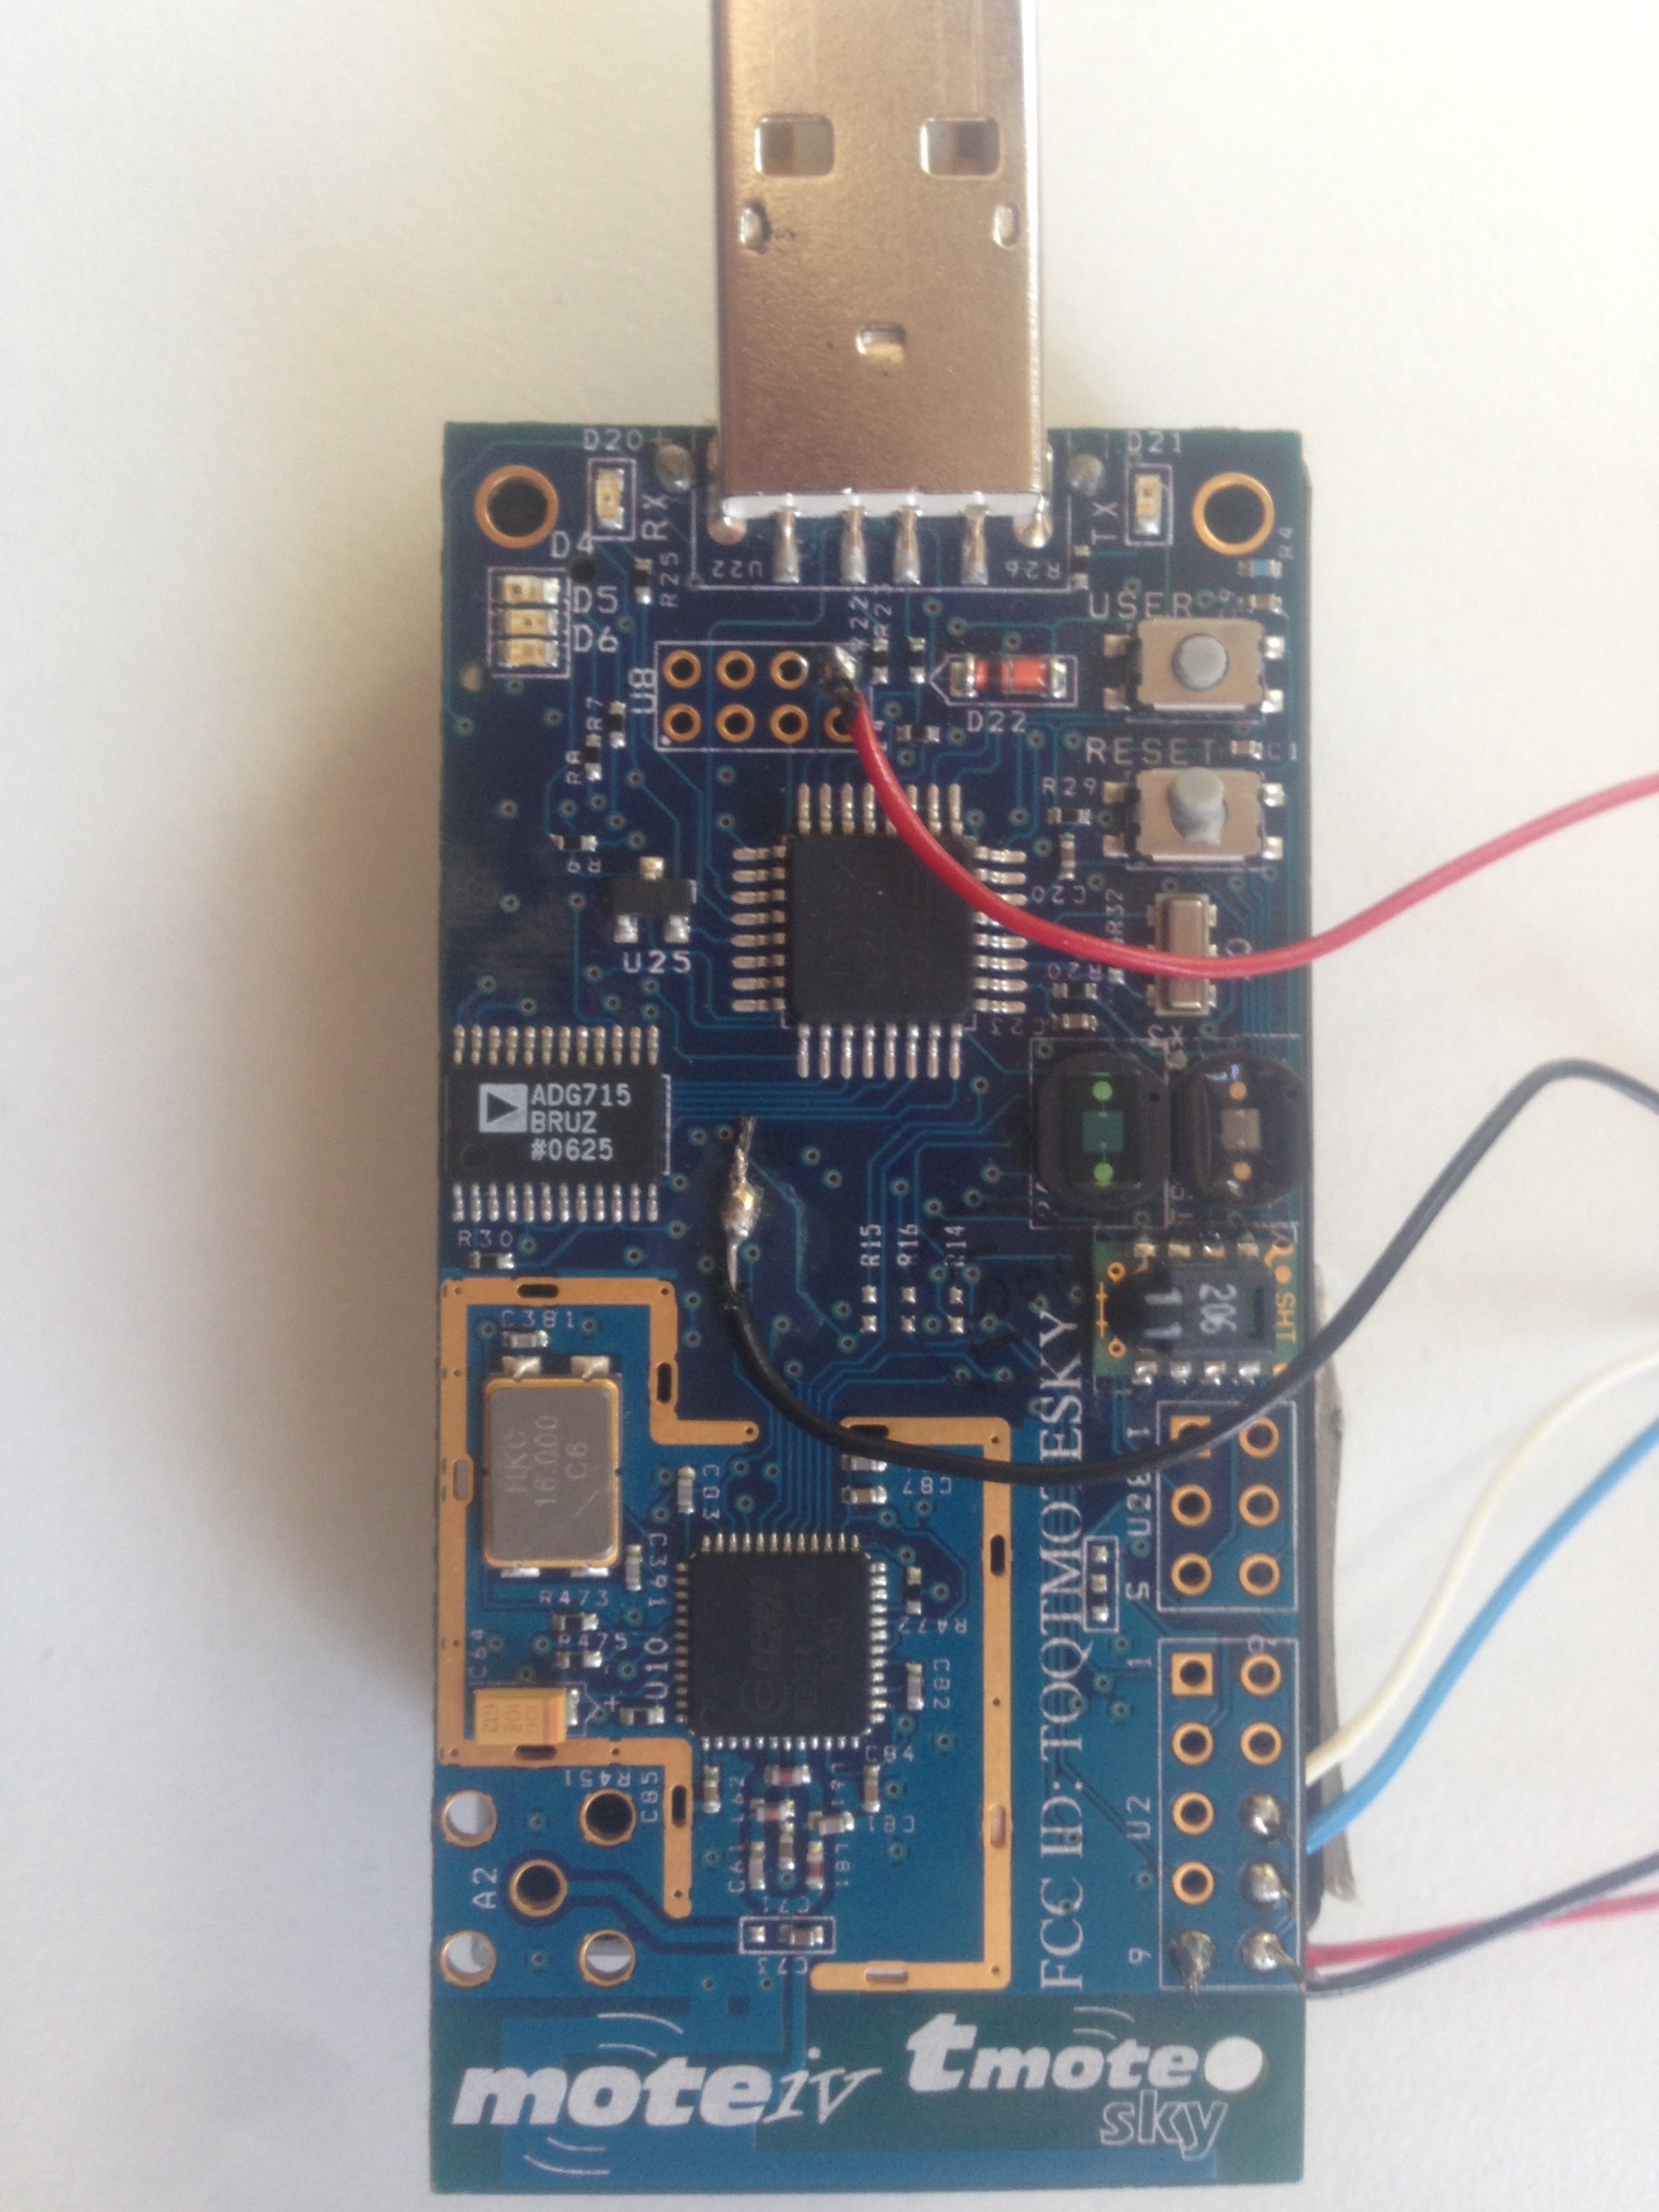
\includegraphics[height=0.45\textwidth]{img/Tmote}
			  \caption{One of the Tmote Sky modules used in the project.}
			  \label{fig_Tmote}
			\end{figure}
	\subsection{Implementation}
		\subsubsection{Connecting the modules}
			The \gls{uwb} modules used in this project have a \gls{spi} that was used for communication with the Tmote Sky modules. Since the Tmote Sky does not have a dedicated \gls{spi} connection through extension pins it had to be connected in another way. In this project it was done as shown in Figure \ref{fig_Tmote_connections} where the $SPI\_MISO$ was connected to a point in the middle of the circuit board. This was achieved by carefully scraping the surface of the board to expose the copper and then cleaning the area with a flux pen before soldering.
			\begin{figure}[H] 
			  \centering
			      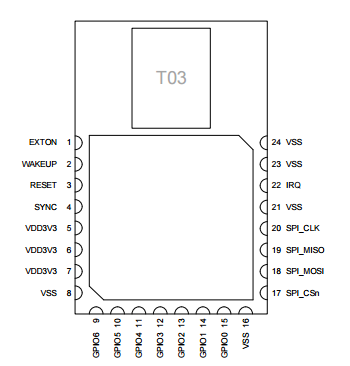
\includegraphics[height=0.6\textwidth]{img/UWB-pinout}
			  \caption{A diagram showing the pins for the DWM1000 UWB module.}
			  \label{fig_UWB_pins}
			\end{figure}
			\begin{figure}[H] 
			  \centering
			      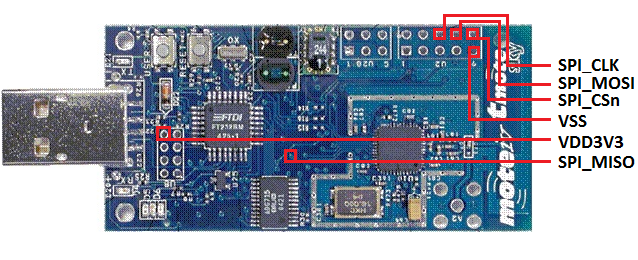
\includegraphics[height=0.45\textwidth]{img/Tmote-connections}
			  \caption{A figure showing how an \gls{uwb} module is connected to a Tmote Sky.}
			  \label{fig_Tmote_connections}
			\end{figure}
			Figure \ref{fig_Tmote_UWB} shows the result after soldering the components according to Figure \ref{fig_UWB_pins} and \ref{fig_Tmote_connections}.
			\begin{figure}[H] 
			  \centering
			      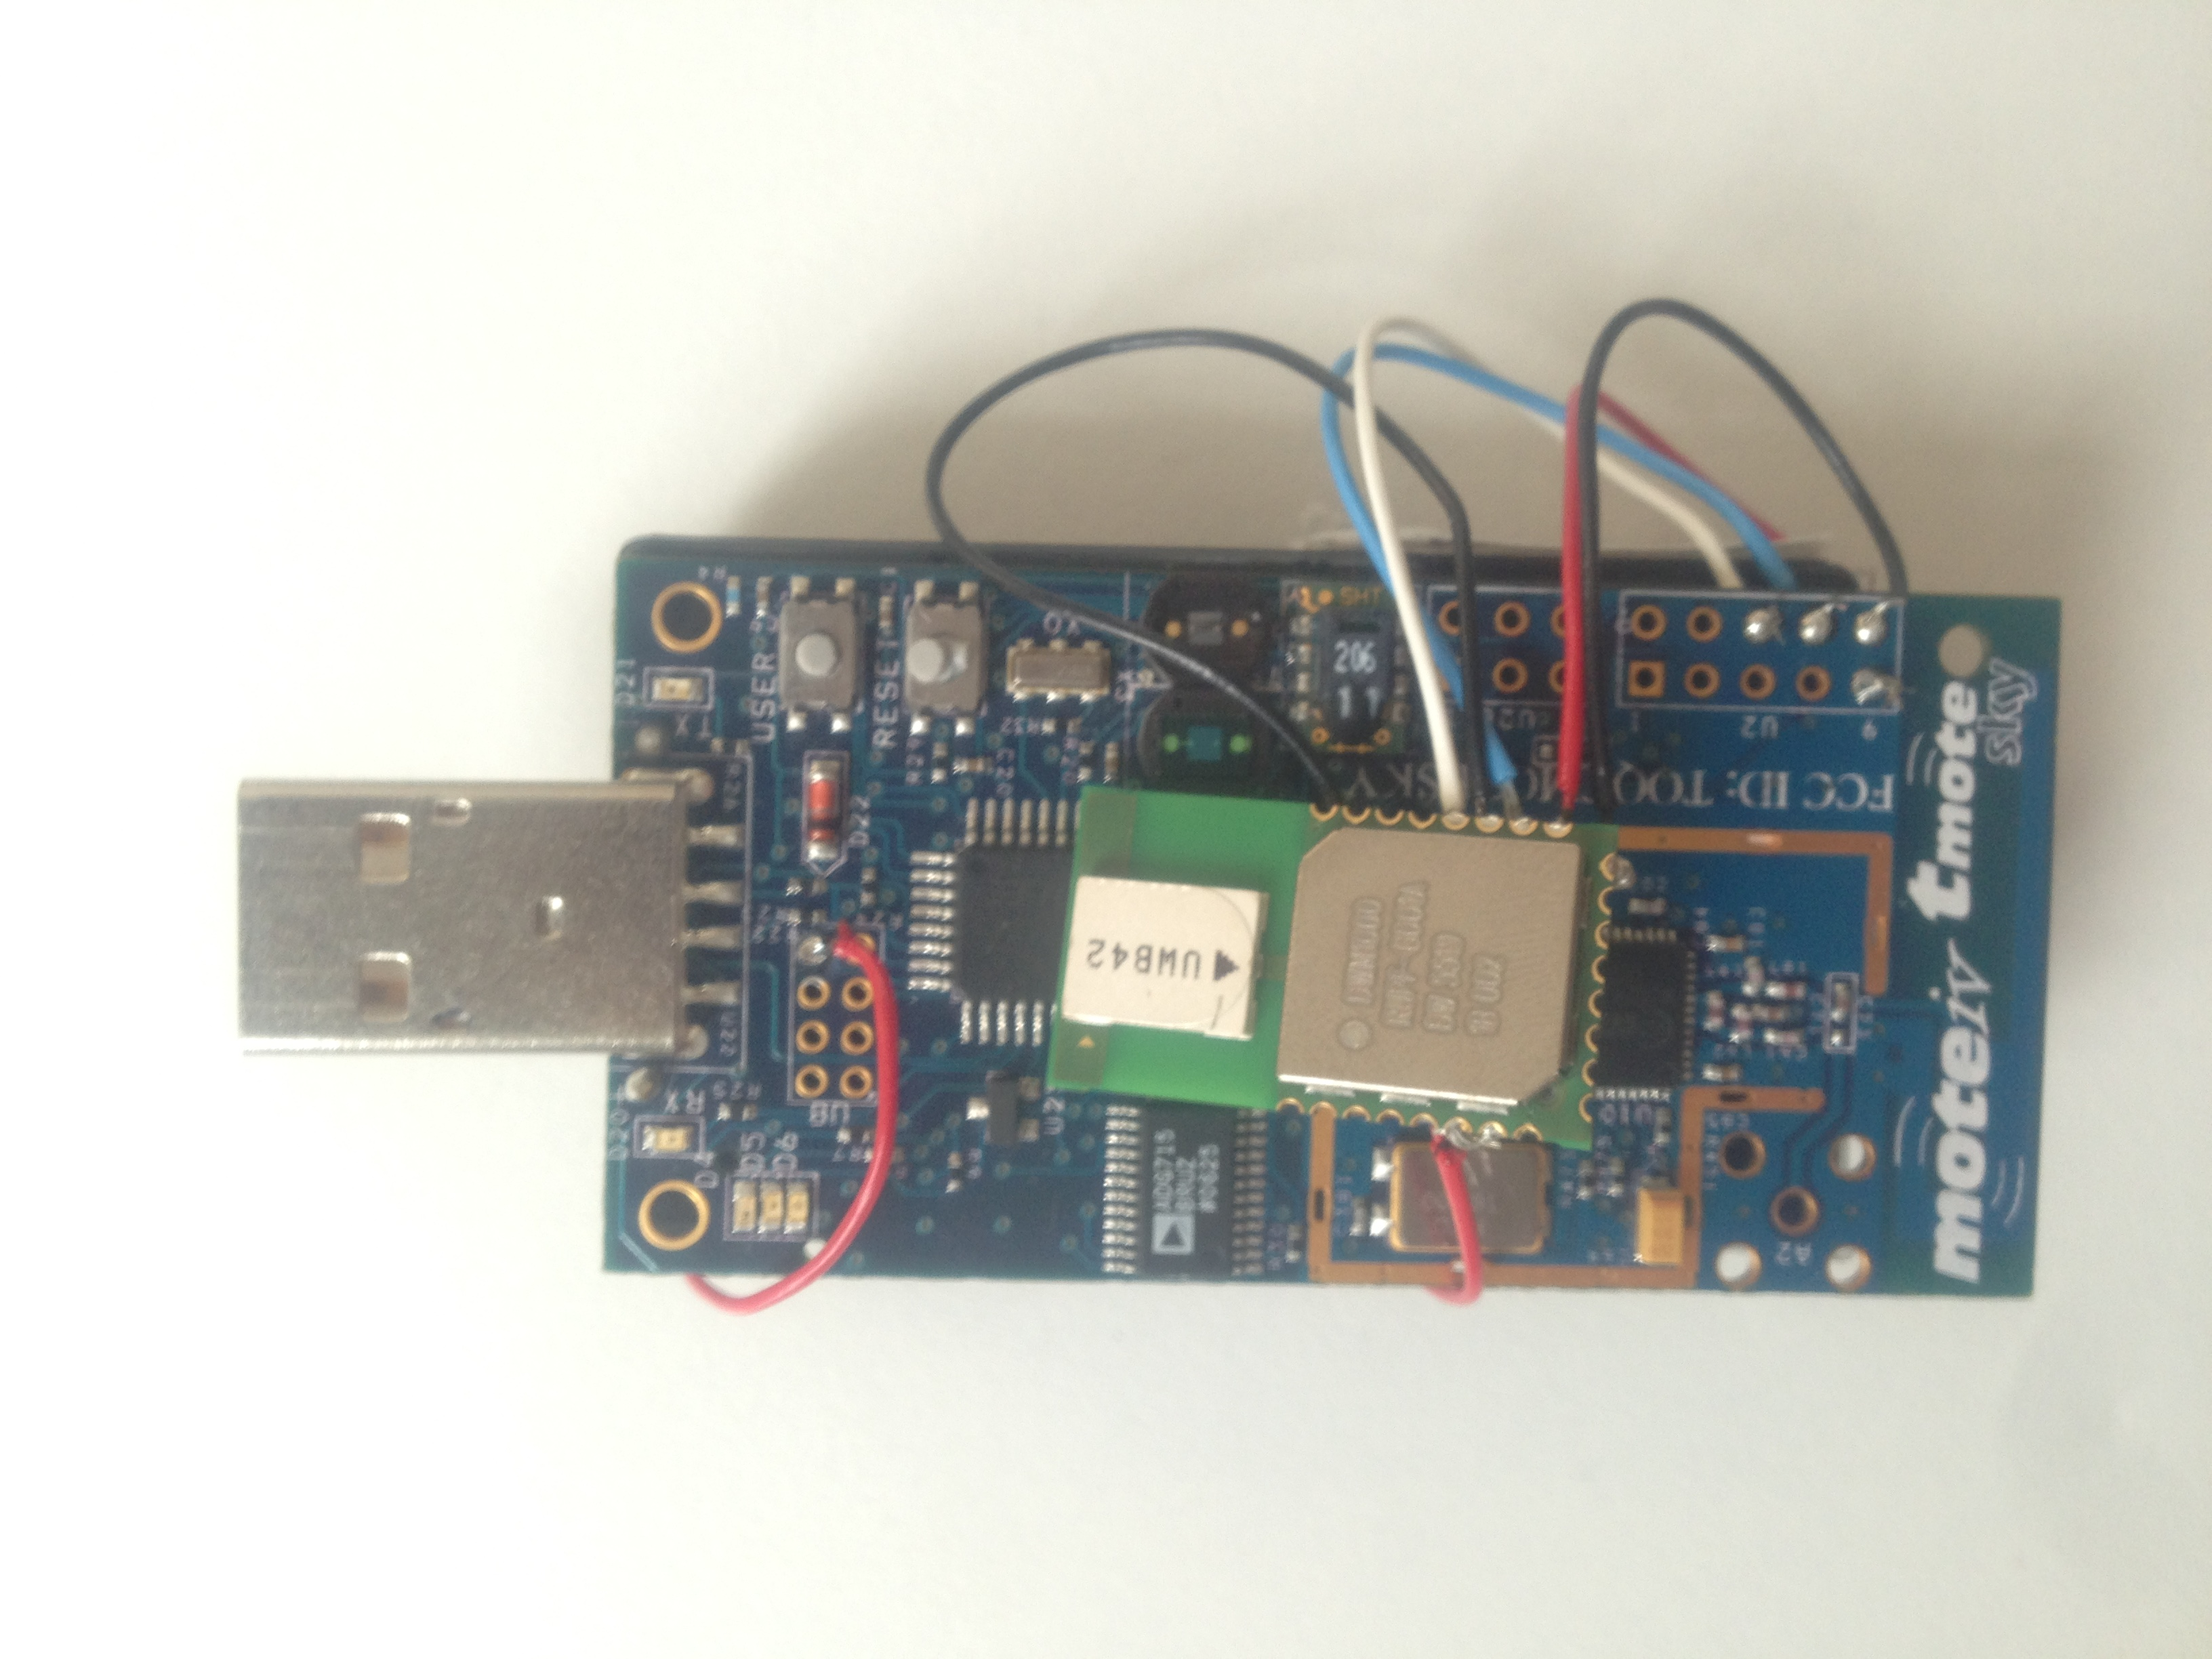
\includegraphics[height=0.45\textwidth]{img/Tmote-UWB}
			  \caption{A figure showing a Tmote Sky connected to a \gls{uwb} module.}
			  \label{fig_Tmote_UWB}
			\end{figure}
		\subsubsection{RSSI}
		The model used to calculate the distance is derived from equation \ref{eq_rssidist} described in \cite{seidel_914_1992} where $\overline{PL}$ denotes mean path loss, $d_0$ denotes a reference distance, $d$ denotes the distance between the transmitter and the receiver and $n$ denotes the path loss exponent. 
		\begin{equation} \label{eq_rssidist}
		\overline{PL}(d) = PL(d_0) + 10 * n * log_{10}(\frac{d}{d_0})
		\end{equation}

		Oguejiofor proposes a model where $d_0$ is one meter and utilizes equation \ref{eq_rssidist} to derive equation \ref{eq_rssidist2} where $n$ is the path loss exponent, $RSSI$ is the received signal strength and $PL(d_0)$ is the path loss at the reference distance of one meter away from the transmitter \cite{oguejiofor_trilateration_2013}. 
		\begin{equation} \label{eq_rssidist2}
		d = 10^{\frac{PL(d_0)-RSSI}{n*10}}
		\end{equation}

		Equation \ref{eq_plexp} was used to determine the value of the path loss exponent, $n$, using $M$ measurements as proposed by Oguejiofor \cite{oguejiofor_trilateration_2013}.
		\begin{equation} \label{eq_plexp}
		n = \frac{\sum_{i=1}^{M}[PL(d_i)-PL(d_0)]}{\sum_{i=1}^{M}[10*log_{10}(d_i)]}
		\end{equation}

		\todo{Rewrite this and maybe move it to theory! \ldots}
		\subsubsection{API}
		\subsubsection{Lab setup}
\clearpage